
%(BEGIN_QUESTION)
% Copyright 2007, Tony R. Kuphaldt, released under the Creative Commons Attribution License (v 1.0)
% This means you may do almost anything with this work of mine, so long as you give me proper credit

In this process, two chemical streams are mixed together in a reactor vessel.  The ensuing chemical reaction is exothermic (heat-producing) and must be cooled by a water cooling system to prevent overheating of the vessel and piping.  A temperature transmitter (TT) senses the reaction product temperature and sends a 4-20 mA signal to a temperature indicating controller (TIC).  The controller then sends a 4-20 mA control signal to the temperature valve (TV) to throttle cooling water flow:

$$\includegraphics[width=15.5cm]{i02933x01.eps}$$

Suppose operators decide to increase production in this process reactor.  This means the incoming feed flow rates will be increased, producing more heat.

\vskip 10pt

Describe in detail how the cooling system will respond to this change in process operations.

\underbar{file i02933}
%(END_QUESTION)





%(BEGIN_ANSWER)

The controller should still be able to maintain the process temperature at setpoint, but it will have to open the cooling water valve further than usual to do so.

%(END_ANSWER)





%(BEGIN_NOTES)

\vskip 20pt \vbox{\hrule \hbox{\strut \vrule{} {\bf Virtual Troubleshooting} \vrule} \hrule}

This question is a good candidate for a ``Virtual Troubleshooting'' exercise.  Presenting the diagram to students, you first imagine in your own mind a particular fault in the system.  Then, you present one or more symptoms of that fault (something noticeable by an operator or other user of the system).  Students then propose various diagnostic tests to perform on this system to identify the nature and location of the fault, as though they were technicians trying to troubleshoot the problem.  Your job is to tell them what the result(s) would be for each of the proposed diagnostic tests, documenting those results where all the students can see.

During and after the exercise, it is good to ask students follow-up questions such as:

\begin{itemize}
\item{} What does the result of the last diagnostic test tell you about the fault?
\item{} Suppose the results of the last diagnostic test were different.  What then would that result tell you about the fault?
\item{} Is the last diagnostic test the best one we could do?
\item{} What would be the ideal order of tests, to diagnose the problem in as few steps as possible?
\end{itemize}

%INDEX% Basics, control loop troubleshooting: determining effect of process load change

%(END_NOTES)


